\chapter{Resultados y discusión}

En este capítulo se van analizar los resultados  a raíz de repetidas ejecuciones del modo Máquina vs Máquina, en cada una de las combinaciones posibles: Algoritmo vs Maniaco, Algoritmo vs Roca y Algoritmo vs Calling Station. Adicionalmente, se han almacenado los datos de las ejecuciones del modo Patrón vs Patrón, a modo de comparativa entre los tres Patrones.

\section{Toma de medidas}
\label{sec:toma}

Lo primero, se va a declarar las especificaciones del entorno en que se han tomado los resultados, así como las condiciones. El proceso ha seguido los pasos del anexo \ref{ch:anexoc}

\begin{itemize}
\item El motor de juego se ha ejecutado usando el depurador de Visual Studio, con el fin de monitorizar el consumo de memoria y el tiempo de ejecución.
\item El algoritmo y, por tanto, el servidor de REST API se han ejecutado usando RStudio.
\item Tal y como se habia definido en \ref{sec:abstracciones}, el dinero inicial de cada jugador será 10.000 y la ciega grande será 20.
\item Por resticciones en la capacidad de los medios, las pruebas se han ejecutado en tandas de 500 iteraciones.
\item El número de medidas totales que se ha tomado 6000 mediciones, divididas de la siguiente manera:
\begin{itemize}
\item Para cada combinación del modo Algoritmo vs Patrón: 1500 iteraciones
\item Para cada combinación del modo Patrón vs Patrón: 500 iteraciones.
\end{itemize} 
\item La principal medida de valoración de los datos es el beneficio medio por partida. La unidad establecida \cite{chen} para esta medida es ciega grande (\textit{Big blind, bb}por partida $\left[\frac{bb}{partida}\right]$.
\item Los valores de beneficio serán representados usando histogramas. \footnote{Un histograma \cite{histo} es un tipo de representación gráfica que agrupa los datos usando intervalos. Para esta representación, se utilizan barras rectangulares verticales cuya altura es proporcional a las frecuencias de dichos intervalos (puede ser tanto frecuencias absolutas,como frecuencias relativas y frecuencias relativas porcentuales).}
\item Adicionalmente, se ha hecho el estudio del victorias y derrotas, así como su desglose a lo largo de las rondas jugadas, para los datos del modo Algoritmo vs Patrón.
\item Se realiza el estudio de los Cuartiles para el modo Algoritmo vs Patrón.
\end{itemize} 

\section{Transformación de las mediciones}

Una vez obtenidos todos los resultados, ha sido necesario hacer una transformación de datos para poder procesarlos adecuadamente con una hoja de cálculo. Al final de cada iteración, se ha almacenado el resultado de la ronda en un fichero .txt, incluyendo el beneficio del jugador[0] de dicha partida.
\begin{figure}[h]
\centering
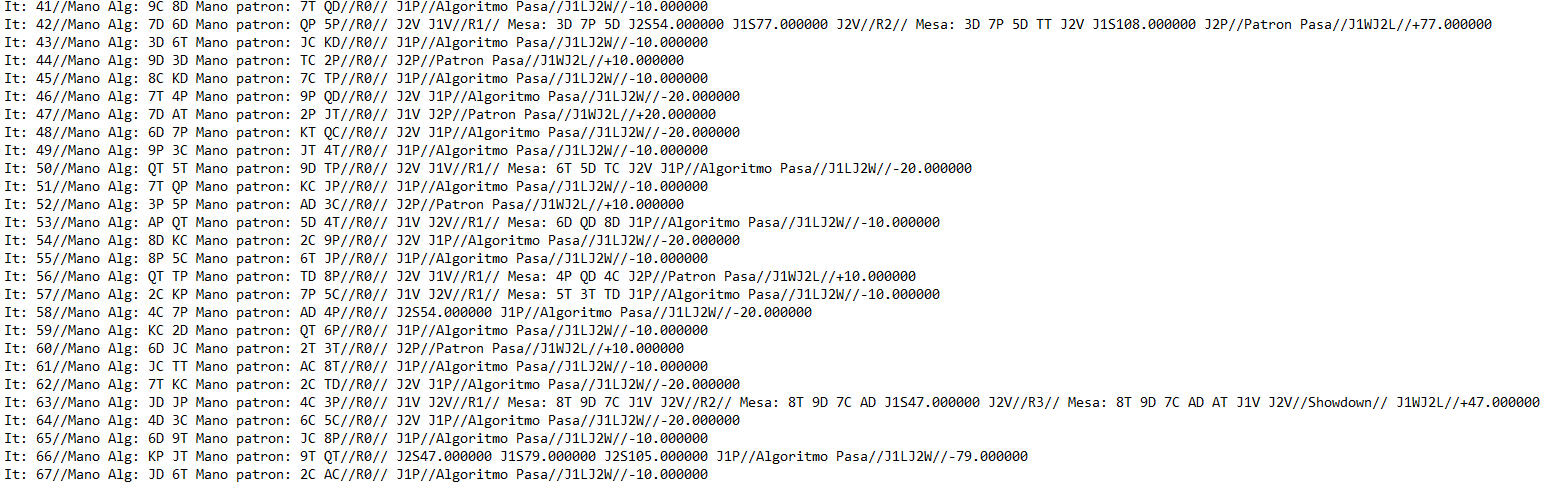
\includegraphics[width=1\textwidth]{figuras/resultados.png}   
\caption{Ejemplo del formato en que se generan los datos}
\label{fig:resultados}
\end{figure}

La idea en que se ha hecho el registro de los datos en el formato explicado en la descripción de los modos del apartado \ref{sec:pokersimu} ha sido para facilitar la transformación y el tratamiento de los datos, ya que al tener un delimitador personalizado (//), permite ser importado por hojas de cálculo de manera bastante eficiente. Un ejemplo de cómo se ven los resultados en bruto se puede ver en \ref{fig:resultados}.

Una vez aplicada una división de columna por delimitador en cada aparición del delimitador, es necesario hacer algunos cambios más\footnote{Cabe destacar que la transformación se ha realizado utilizando Microsoft Excel 2019.Se desconoce si es necesario hacer pasos adicionales o si algunos pasos no son necesarios en caso de que se utilicen otras herramientas para el tratamiento de los datos.}
Debido a que se van añadiendo // con cada ronda, eso implica que se tenga un rellenado de columnas irregular, ya que solamente las rondas en las que se haya alcanzado el River o el Showdown rellenarán por completo todas las columnas, mientras que el resto las rellenarán con un valor \textit{NULL}.  Por lo que es necesario agrupar el resultado de la ronda en una sola columna, para su procesado.

Para esto, se añade una columna condicional en la cual se añadirán cláusulas del tipo \textit{Si(Columna[n]$\neq$NULL)-$>$valor}, tal y como se muestra en la imagen \ref{fig:tf1}. Por el diseño del registro, los valores se almacenan en una diferencia de 2 separaciones, con un máximo de 6 separaciones (entre un resultado del preflop y un resultado del River/Showdown).
\begin{figure}[h]
\centering
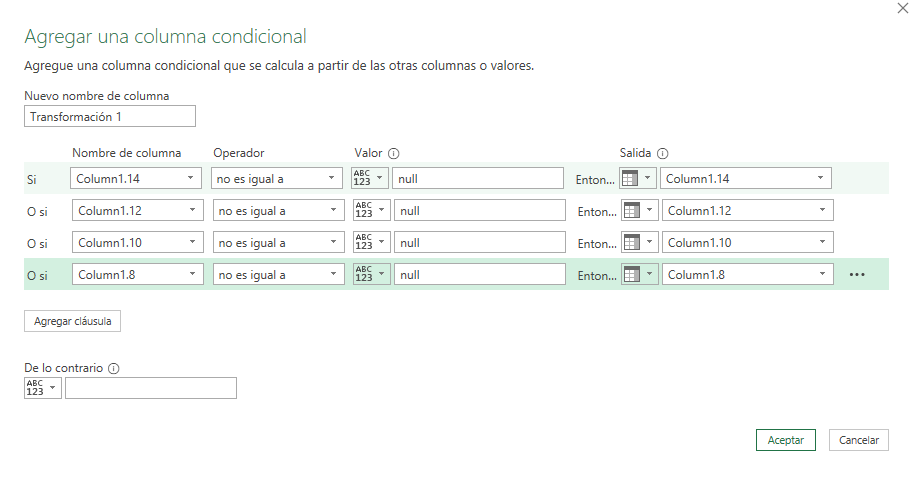
\includegraphics[width=1\textwidth]{figuras/transformacion1.png}   
\caption{Ejemplo de las cláusulas de la columna condicional en la transformación de datos}
\label{fig:tf1}
\end{figure}

Una vez unificados todos los resultados en una misma columna, se ha necesitado hacer 3 transformaciones más:

\begin{enumerate}
\item Conversión de tipo de la columna condicional: debido a que el tipo de importación ha sido desde texto/csv, el tipo de dato estaba definido como texto, por lo que se transforma el tipo de dato en numérico.
\item Reducción de escala: Debido a que los valores de apuesta en el motor de juego eran un tipo de variable float, a la hora de almacenarlos en el registro ha almacenado estos 6 decimales. El problema se ha generado por la diferencia de notación a la hora de escribir los decimales entre Excel y Visual Studio: Visual estudio utiliza "." para comenzar la numeración decimal, mientras que excel utiliza "," y tiene codificado que un "." se utiliza como separación de millares, por lo que al hacer laconversión, se tiene que la columna de resultados está multiplicada por $10^6$, por lo que ha sido necesario crear una nueva columna cuyo valor sea la dicisión del valor de esta columna condicional entre $10^6$. Esta columna es el Beneficio Neto, o resultado Neto, de cada una de las manos de ese registro.
\item Cambio de unidades de Resultado Neto: Tal y como se ha mencionado en el apartado \ref{sec:toma}, la unidad establecida del beneficio es la ciega grande (\textit{ BB}), por lo que para tener el resultado en esta unidad es necesario dividir el resultado Neto por el valor de \textit{BB}. Tal y como se especificó en el apartado \ref{sec:abstracciones}, la ciega grande tiene un valor de 20 para todas las tomas de datos, por lo que se añadirá una última columna como división del valor de Beneficio Neto/20.
\end{enumerate}

Esta última columna, Resultado (BB), será la utilizada de cara a los cálculos y el análisis de los datos.

Una vez realizada la transformación de todos los datos, se procede al estudio de los mismos.

\section{Modo Patrón vs Patrón}
\label{sec:pvp}

En este apartado se van a exponer los resultados de los datos obtenidos. Cabe destacar que, aunque las medidas hayan sido 500 por cada combinación de dos patrones, cada uno de los tres patrones ha participado en 1000 medidas: 500 como jugador[0] y 500 como jugador[1].

Ya que el, por las abstracciones que se tomaron a la hora de plantear el diseño (vease apartado \ref{sec:abstracciones} las partidas son un juego Suma-Cero, si un jugador tiene una ganancia X, el otro jugador tiene una pérdida X. Es decir, el resultado de un jugador es el opuesto del resultado del otro jugador.

Por tanto, para el estudio de cada uno de los patrones, realmente se han utilizado un total de 1000 valores: los valores en los que ese patrón ha sido jugador[0] y el opuesto de los valores en los que ese patrón ha sido jugador[1].

Para este estudio, una vez obtenidos los datos se han calculado la media ($\bar{x}$), varianza($\sigma^2$), desviación típica ($\sigma$) y coeficiente de variación (C.V.)

\subsection{Maniaco}

Este patrón, caracterizado por la agresividad a la hora de jugar y como acción predominante Subir ha obtenido unos resultados bastante positivos frente a los otros patrones.



\begin{figure}[h]
\centering
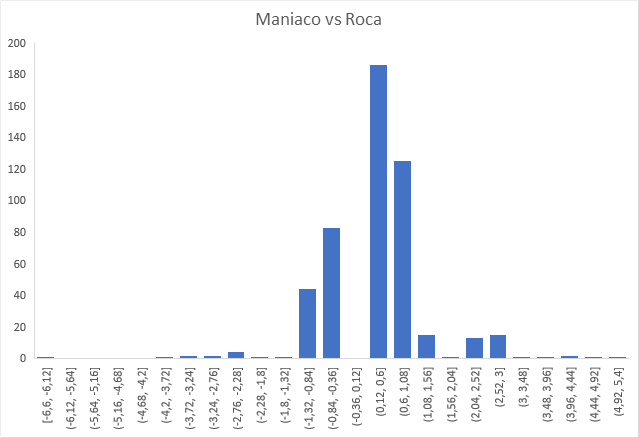
\includegraphics[width=1\textwidth]{figuras/MvR.png}   
\caption{Gráfica Maniaco vs Roca}
\label{fig:MvR}
\end{figure}

\begin{figure}[h]
\centering
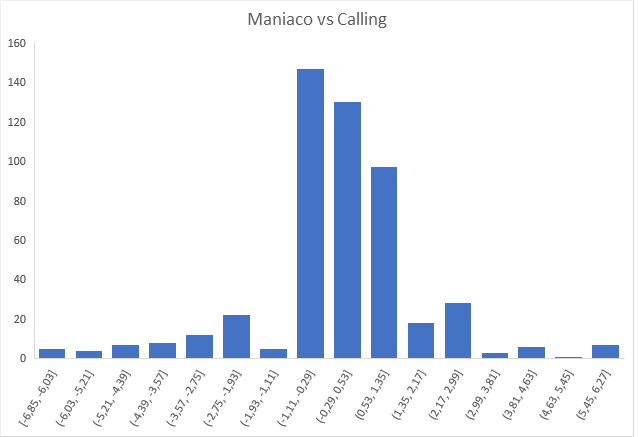
\includegraphics[width=1\textwidth]{figuras/MvC.png}   
\caption{Gráfica Maniaco vs Calling Station}
\label{fig:MvC}
\end{figure}

\begin{figure}[h]
\centering
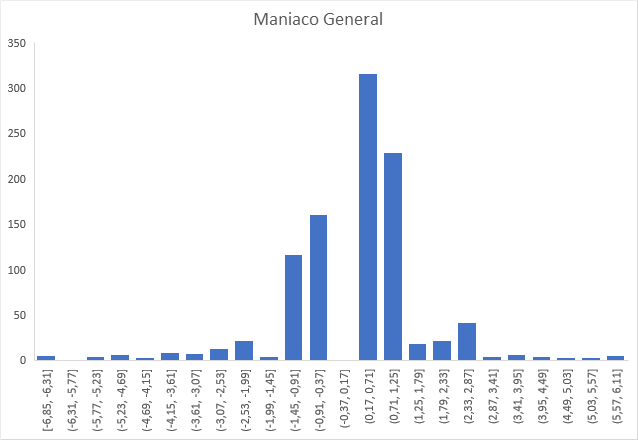
\includegraphics[width=1\textwidth]{figuras/MG.png}   
\caption{Gráfica de Resultados de Maniaco Patrón vs Patrón}
\label{fig:MGR}
\end{figure}

\begin{longtable}[c]{lrrr}
\hline
Maniaco & Vs Roca & Vs Calling & General \\ \hline
$\bar{x}$ & 0,4257 & 0,0434 & 0,23455 \\ 
$\sigma^2 $& 1,19822095 & 3,46452549 & 2,36561441 \\ 
$\sigma$ & 1,09463279 & 1,86132359 & 1,5380554 \\
C.V. & 2,57137137 & 42,8876402 & 6,55747346 \\ \hline
\end{longtable}

El resultado final del patrón Maniaco es $0,23455\pm1,5380554$ $\frac{bb}{partida}$.

Al observar estos datos, se puede deducir que este patrón es el que ha obtenido el mejor resultaado por encima de los otros dos, ya que es el único que tiene una media positiva, tanto contra otros patrones como el resultado general. También es el patrón con la desviación más alta de los tres por lo que los resultados esperados del patrón maniáco tienen mayor rango (pudiendo generar ganancias mayores, pero también pérdidas de mayor cantidad).

\newpage

\subsection{Roca}

Estos son los resultados del patrón Roca, el más pasivo que los demás, teniendo como acción predominante pasar, por lo que acaba jugando muy pocas manos pero las pocas que juega son porque tiene una mano buena.

\begin{figure}[h]
\centering
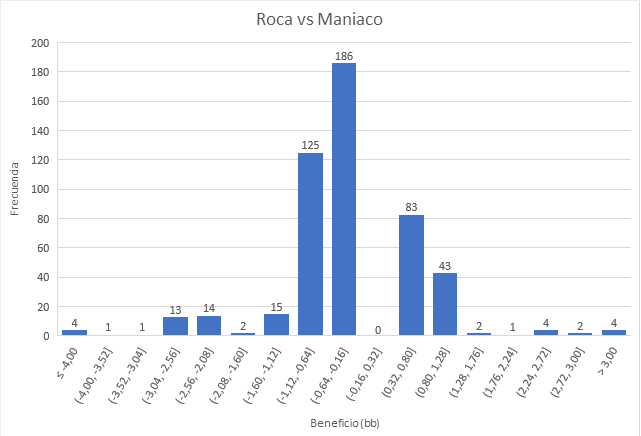
\includegraphics[width=1\textwidth]{figuras/RvM.png}   
\caption{Gráfica Roca vs Maniaco}
\label{fig:RvM}
\end{figure}

\begin{figure}[h]
\centering
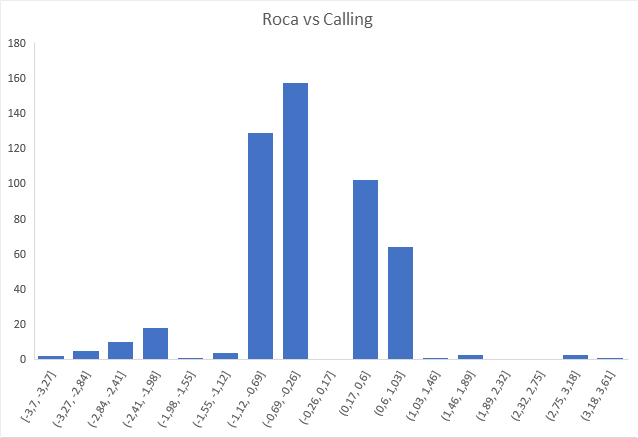
\includegraphics[width=1\textwidth]{figuras/RvC.png}   
\caption{Gráfica Roca vs Calling Station}
\label{fig:RvC}
\end{figure}

\begin{figure}[h]
\centering
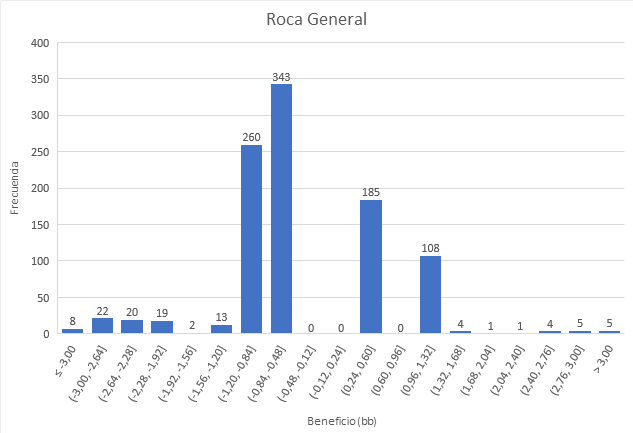
\includegraphics[width=1\textwidth]{figuras/RG.png}   
\caption{Gráfica de Resultados de Roca  Patrón vs Patrón}
\label{fig:RGR}
\end{figure}


\begin{longtable}[c]{lrrr}
\hline
Roca & vs Calling & vs Maniaco & General \\ \hline
$\bar{x}$ & -0,3371 & -0,4257 & -0,3814 \\
$\sigma^2$ & 0,95773406 & 1,19822095 & 1,0788629 \\ 
$\sigma$ & 0,97863888 & 1,09463279 & 1,03868325 \\ 
C.V. & -2,90311148 & -2,57137137 & -2,72334361 \\ \hline
\end{longtable}

El resultado final del patrón Roca es $-0,3814\pm1,03868325$ $\frac{bb}{partida}$.

\smallskip

Observando estos datos, se puede deducir que este patrón es el que ha obtenido el peor valor de media de los 3 (siendo el único que tiene una media general negativa).También es el patrón con la desviación más pequeña de los tres, lo que significa que es el patrón que presenta los datos más compactos.

\clearpage

\subsection{Calling Station}

Aquí se presentan los datos del patrón Calling station, un patrón intermedio entre ambos, pues su acción predominante es ver la apuesta, lo que significa que acaba jugando más apuestas, pero no mete la presión de un maniaco.

\begin{figure}[h]
\centering
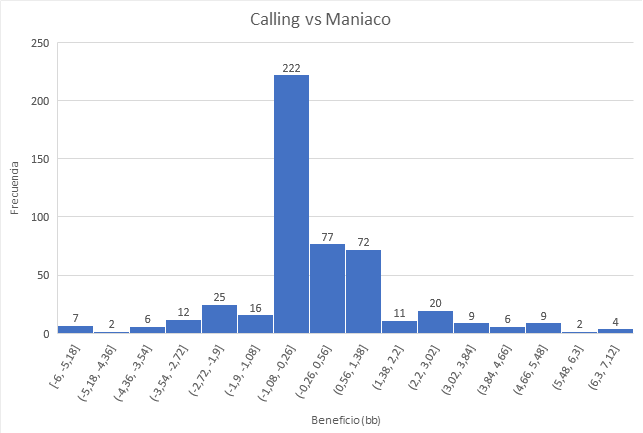
\includegraphics[width=1\textwidth]{figuras/CvM.png}   
\caption{Gráfica Calling Station vs Maniaco}
\label{fig:CvM}
\end{figure}

\begin{figure}[h]
\centering
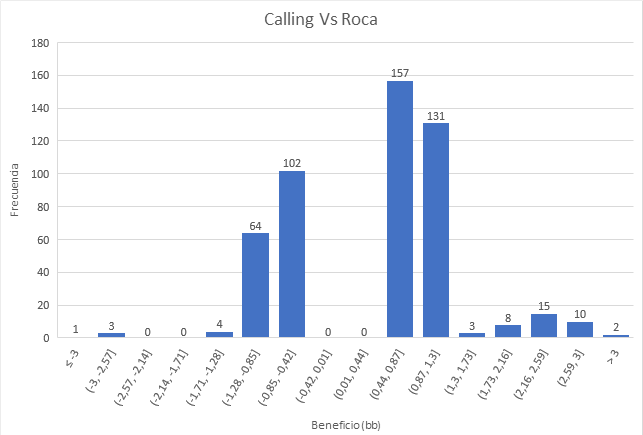
\includegraphics[width=1\textwidth]{figuras/CvR.png}   
\caption{Gráfica Calling Station vs Roca}
\label{fig:CvR}
\end{figure}

\begin{figure}[h]
\centering
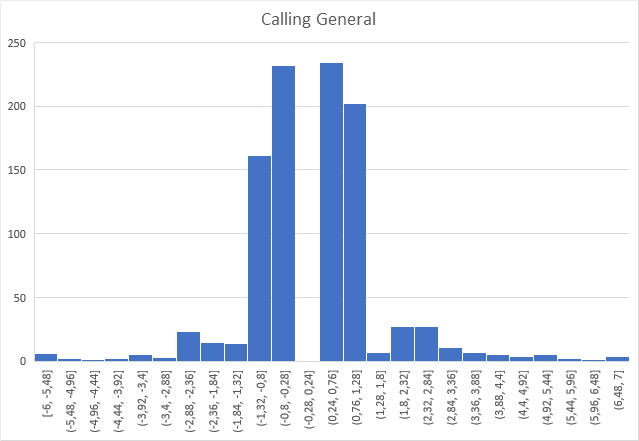
\includegraphics[width=1\textwidth]{figuras/CG.png}   
\caption{Gráfica de Resultados de Calling Station Patrón vs Patrón}
\label{fig:CGR}
\end{figure}

\begin{longtable}[c]{lrrr}
\hline
Calling Station & Vs Maniaco & vs Roca & General \\ \hline
$\bar{x}$ & -0,0434 & 0,3371 & 0,14685 \\ 
$\sigma^2$ & 3,46452549 & 0,95773406 & 2,24514773 \\ 
$\sigma$ & 1,86132359 & 0,97863888 & 1,4983817 \\ 
C.V. & -42,8876402 & 2,90311148 & 10,2034845 \\ \hline
\end{longtable}


El resultado final del patrón Calling Station es $ 0,14685\pm1,4983817$  $\frac{bb}{partida}$.

\smallskip

Observando estos datos, se puede razonar que este patrón tiene unos resultados mixtos, pues si bien tiene una media posivita, su media es menor que la de Maniaco, y su desviación media es menor que la de Maniaco también, pero bastante cercana, lo cual no convierte sus datos en un conjunto tan compacto como lo sería un jugador más defensivo.

\clearpage

\subsection{Discusión sobre los datos obtenidos en el modo Patrón vs Patrón}

Se agrupan los resultados finales en este apartado, para poder hacer una comparación más sencilla entre los 3

\vspace{5mm} %5mm vertical space

Maniaco:  $0,23455\pm1,5380554$ $\frac{bb}{partida}$.

Roca: $-0,3814\pm1,03868325$ $\frac{bb}{partida}$.

Calling Station: $ 0,14685\pm1,4983817 $ $\frac{bb}{partida}$.

\vspace{5mm} %5mm vertical space
Estos datos son los esperados en esta comparació entre patrones, pues si únicamente se mantiene una de las 3 acciones posibles como predominante, Maniaco genera más victorias y más rentabilidad, pues la presión que ejerce con las constantes subidas hace que muchos oponentes pasen una mano por miedo a que tenga una buena mano. Las subidas constantes provocan también un aumento de la varianza y, por tanto, de la desviación, pues hay mayor dinero apostado, lo que significa que las variaciones de dinero también serán mayores.

En el extremo opuesto del espectro se encontraría el jugador defensivo, en este caso, Roca. Pues sus estrategias hacen que, si bien el número de apuestas perdidas aumente, las pocas que  juege seguramente las gane. Al participar tan poco en las apuesas, provoca una desviación mucho menor, ya que, al intentar minimizar pérdidas jugando defensivo, tampoco se pueden llegar a generar ganancias. 

Y el resultado intermedio lo tiene con Calling Station, donde tiene tanto lo peor de ambos como lo mejor de ambos: si bien juega muchas apuestas, hay menos jugadas que gane a base de intimidar, lo que provoca que su media sea menor que la de Maniaco. También cabe mencionar que, ya que prácticamente siempre ve la  apuesta, su mero comportamiento hace que las apuestas no suban tanto, aunque si que permite que suban.

De estos datos se puede deducir que mantener una única estrategia defensiva no acaba siendo tan beneficioso que una agresiva. También se puede obtener de estos datos que todos tienen cosas favorables y perjudiciales, por lo que sería lógico pensar que mantener siempre una mísma estrategia acaba siendo perjudicial, pues, a la larga, los jugadores acaban adaptándose al ritmo de subidas, forzando algunas pérdidas. Pero en pocos juegos, acaba siendo más ventajosa maniaco.

\section{Modo Algoritmo vs Patrón}


En este apartado se procede a analizar los datos obtenidos por el Modo Algoritmo vs Patrón, primero analizándolos inidividualmente con cada patrón y, posteriormente, con el cómputo total de los datos de este modo, para obtener el resultado del experimento.

A diferencia del modo Patrón vs Patrón, aquí se analizarán tanto los Cuartiles $Q_1$, $Q_2$, $Q_3$, que corresponden a los percentiles $P_{25}$, $P_{50}$, $P_{75}$, así como el estudio de las victorias.

\subsection{Discusión previa y explicación de las medidas}
\label{sec:predisc}

En este caso, los datos de los que dispone y su exposición puede que no sean de todo intuitivos. Inicialmente se tomaron 2 medidas de datos del algoritmo enfrentándose a cada uno de loa patrones (que son G1 y G2), pero al hacer un análisis previo de estos datos, se llegó a la conclusión de que había algo que no rondaba bien. Esto que se detecto fue que, en unas cuantas rondas en las que, aun teniendo todos los datos a favor, el algoritmo pasaba la apuesta.

Siguiendo los datos de depurador y del servidor API, los cálculos eran correctos, pero esa decisión no era problema del algoritmo, sino de que el valor que aleatorizaba la salida habia sacado un valor prácticamente 0, por lo que se generó el "Pasar"

Si bien esa era una de las premisas iniciales del proyecto (que el algoritmo fuera, en parte, imprevisible), en este punto esta premisa puede no ser tan acertada. Por lo que se decidió probar a tomar medidas eliminando dicho factor aleatorio y dejando únicamente la opción con más peso (manteniendo la probabilidad de hacer faroles de la misma manera que estaba diseñada). 
Con esta modificación se generó una tanda de datos para cada patrón (GE).

Para poder hacer una comparación adecuada y un total del enfrentamiento contra cada patrón, lo planteado era repetir las dos tandas de datos, pero por imposibilidades físicas se pudo realizar la segunda toma con el motor de juego modificado. 

Por lo que los datos de los que se dispone es G1, G2 y G3. 

Puesto que se va a aprovechar y utilizar estos datos para hacer una comparativa del total del funcionamiento, es necesario ponderar para la agrupación de datos (T). De no hacerlo, los resultados con el factor aleatorio tendrían un peso del 66.67\% sobre el total.

Por este motivo, se aplicará un modificador de 0.5 a los datos G1 y G2 \textbf{solamente para los cálculos de T} . Para las comparativas de histogramas, Cuartiles, y los valores descriptivos estadísticos individuales, se tomará el valor original.

\subsection{Estudio del enfrentamiento individual de Algoritmo vs Patrón}
\label{sec:AvP}

En este apartado, se expondrán los datos de los enfrentamientos de manera individual, sin tener en consideración los datos de losenfrentamientos con otros patrones. 

\subsubsection{Algoritmo vs Maniaco}

Se procede a desarrollar el resultado de las dos iteracciones con Maniaco, empezando por los resultados de beneficio

\begin{longtable}[c]{lrrrr}
\hline
Algoritmo vs Maniaco & G1 & G2 & GE & T \\ \hline
$\bar{x}$ & -0,4847 & -0,3566 & -0,2881 & -0,37646667 \\ 
$\sigma$ & 1,468904663 & 1,83463251 & 2,49953263 & 1,98251848 \\ 
$\sigma^2$  & 2,15768091 & 3,36587644 & 6,24766339 & 3,93037952 \\ 
C.V. & -3,030543972 & -5,14479111 & -8,67592029 & -5,26611956 \\ 
$Q_1$ & -1,108333333 & -1,04719198 & -1,214375 & -0,73288462 \\
$Q_2$ & -0,648275862 & -0,75707736 & -0,46176471 & -0,30397351 \\ 
$Q_3$ & -0,248029557 & -0,46696275 & 9,77254902 & 0,07475166 \\ \hline
\caption{Tabla Algoritmo vs Maniaco}
\label{tab:AvM}
\end{longtable}


\begin{figure}[h]
\centering
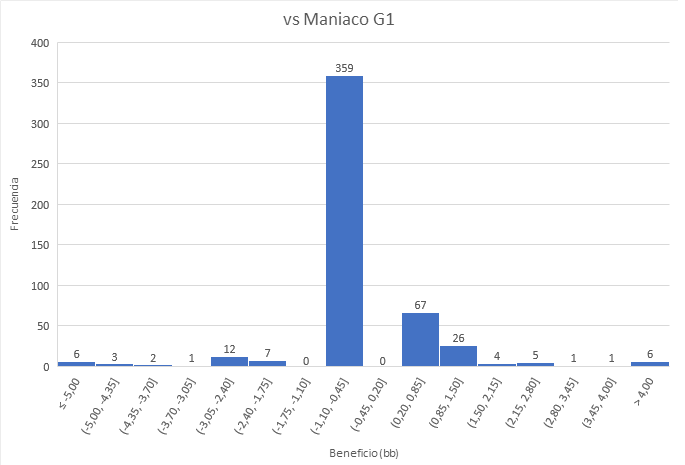
\includegraphics[width=1\textwidth]{figuras/AvMG1.png}   
\caption{Gráfica Algoritmo vs Maniaco (G1)}
\label{fig:AvMG1}
\end{figure}

\begin{figure}[h]
\centering
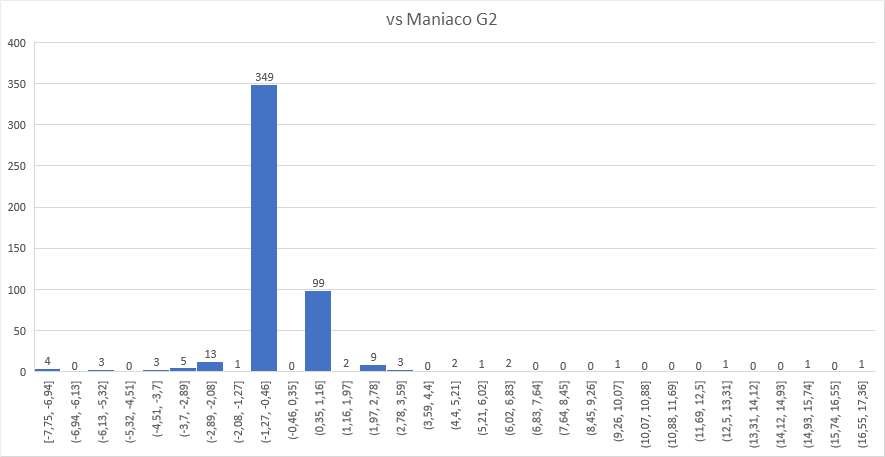
\includegraphics[width=1\textwidth]{figuras/AvMG2.png}   
\caption{Gráfica Algoritmo vs Maniaco (G2)}
\label{fig:AvMG2}
\end{figure}


\begin{figure}[h]
\centering
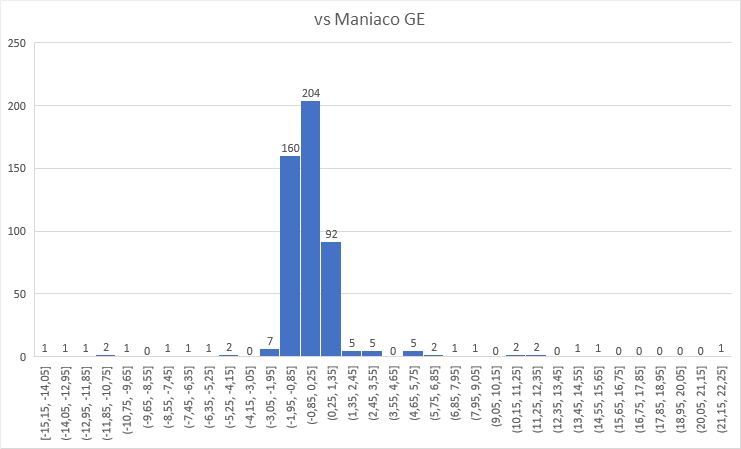
\includegraphics[width=1\textwidth]{figuras/AvMGE.png}   
\caption{Gráfica Algoritmo vs Maniaco (GE)}
\label{fig:AvMGE}
\end{figure}

\begin{figure}[h]
\centering
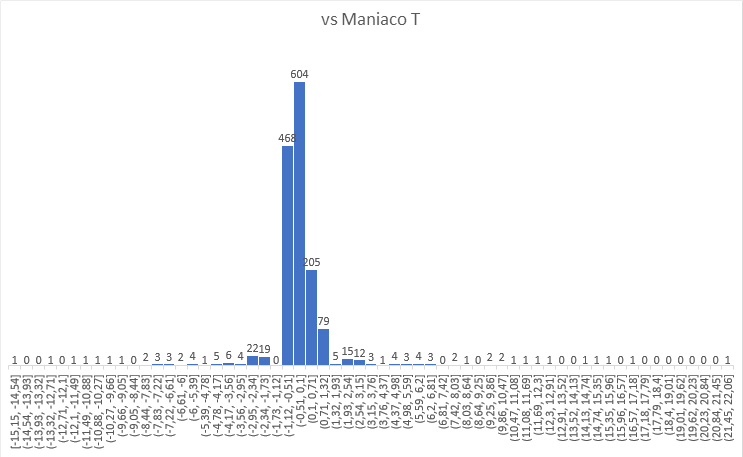
\includegraphics[width=1\textwidth]{figuras/AvMT.png}   
\caption{Gráfica Algoritmo vs Maniaco (T)}
\label{fig:AvMGT}
\end{figure}

\vspace{5mm} %5mm vertical space

Ahora se procede a estudiar el desarrollo de las partidas en cada uno de los conjuntos de los datos, estudiando primero el número de victorias generales, el número de partidas que han acabado en una determinada ronda (y el desglose de victorias/derrotas de esas partidas), así como calcular el porcentaje de victorias respecto a las rondas que acaban en esa ronda.

\vspace{5mm} %5mm vertical space

\begin{longtable}[c]{lrrrr}
\hline
Algoritmo vs Maniaco & G1 & G2 & GE & T \\ \hline
Nº Partidas & 500 & 500 & 500 & 1500 \\ 
Nº Victorias & 110 & 122 & 118 & 350 \\ 
Nº Derrotas & 390 & 378 & 382 & 1150 \\ 
Partidas Fin Preflop & 406 & 410 & 404 & 1220 \\ \
Nº Victorias preflop & 80 & 92 & 71 & 243 \\ 
Nº Derrotas Preflop & 326 & 318 & 333 & 977 \\ 
Partidas Fin Flop & 60 & 57 & 56 & 173 \\ 
Nº Victorias Flop & 15 & 14 & 28 & 57 \\ 
Nº Derrotas Flop & 45 & 43 & 28 & 116 \\ 
Partidas Fin Turn & 23 & 23 & 23 & 69 \\ 
Nº Victorias Turn & 8 & 11 & 10 & 29 \\ 
Nº Derrotas Turn & 15 & 12 & 13 & 40 \\ 
Partidas Fin River & 8 & 4 & 3 & 15 \\ 
Nº VictoriasRiver & 6 & 1 & 0 & 7 \\ 
Nº Derrotas River & 2 & 3 & 3 & 8 \\ 
Partidas Fin Showdown & 3 & 6 & 14 & 23 \\ 
Nº Victorias Swodown & 1 & 4 & 9 & 14 \\ 
Nº Derrotas Showdown & 2 & 2 & 5 & 9 \\ \hline
\caption{Desglose de las partidas contra Maniaco}
\label{tab:PlaysM}
\end{longtable}

\begin{longtable}[c]{lrrrr}
\hline
\% Victoria vs Maniaco & G1 & G2 & GE & T \\ \hline
General & 22,000\% & 24,400\% & 23,600\% & 23,333\% \\ 
Preflop & 19,704\% & 22,439\% & 17,574\% & 19,918\% \\ 
Flop & 25,000\% & 24,561\% & 50,000\% & 32,948\% \\ 
Turn & 34,783\% & 47,826\% & 43,478\% & 42,029\% \\ 
River & 75,000\% & 25,000\% & 0,000\% & 46,667\% \\ 
Showdown & 33,333\% & 66,667\% & 64,286\% & 60,870\% \\ \hline
\caption{Porcentajes de victoria Algoritmo vs Maniaco (Desglose por rondas)}
\label{tab:winrateM}
\end{longtable}

El resultado final del enfrentamiento contra el patrón Maniaco es $-0.3764667\pm1.982518$ $\frac{bb}{partida}$.

\vspace{5mm} %5mm vertical space

Teniendo todos los datos de los enfrentamientos contra Maniaco, se puede encontrar que GE supone una mejora de la media con respecto tanto a G1 y G2. Si buen aumentá la desviación típica, cabe destacar de estos datos el valor de $Q_3$, en el que se puede apreciar un incremento de mas de 10 puntos, lo que significa que el beneficio que se ha obtenido ha sido considerablemente mayor al de G1 y G2. Esto, en el caso de $Q_1$ no ocurre, pues, si bien es cierto que el valor es menor, el descenso no es tan significativo como el incremento de $Q_3$. 
Lo último reseñable de estos datos es el análisis de las victorias. 
Si bien es cierto que las victorias totales no se han incrementado, en concreto son peores que G2, lo que si se ha visto un incremento significativo es el número de las partidas que llegan hasta el showdown, ganando 9 de las 14 partidas. 

\clearpage

\subsubsection{Algoritmo vs Roca}

Se procede a desarrollar el resultado de las dos iteracciones con Roca, empezando por los resultados de beneficio

\begin{longtable}[c]{lrrrr}
\hline
Algoritmo vs Roca & G1 & G2 & GE & T \\ \hline
$\bar{x}$ & -0,188 & -0,1133 & -0,2538 & -0,13481667 \\ 
$\sigma$ & 0,8878415 & 0,90963343 & 0,7136555 & 0,55795976 \\
$\sigma^2$& 0,78826253 & 0,82743298 & 0,50930417 & 0,3113191 \\
C.V. & -4,72256116 & -8,02853865 & -2,81188139 & -4,13865567 \\ 
$Q_1$ & -0,98572581 & -0,62575758 & -0,71976378 & -0,5248427 \\ 
$Q_2$ & -0,34 & -0,37323232 & -0,53306604 & -0,20319338 \\ 
$Q_3$ & 0,37567568 & 0,37068966 & 0,31245614 & 0,345837 \\ \hline
\caption{Tabla Algoritmo vs Roca}
\label{tab:AvR}
\end{longtable}



\begin{figure}[h]
\centering
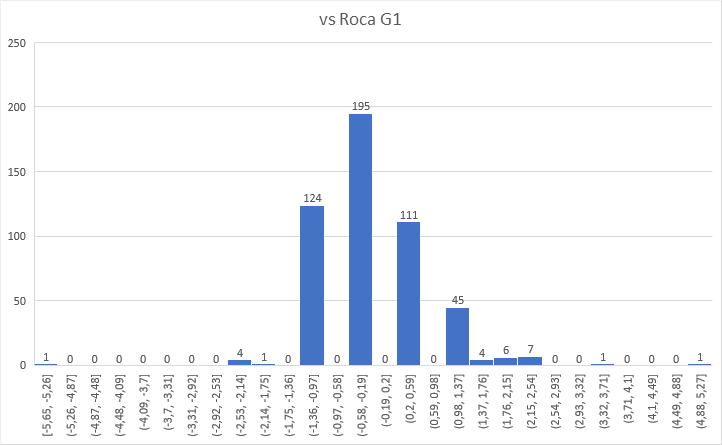
\includegraphics[width=1\textwidth]{figuras/AvRG1.png}   
\caption{Gráfica Algoritmo vs Roca(G1)}
\label{fig:AvRG1}
\end{figure}

\begin{figure}[h]
\centering
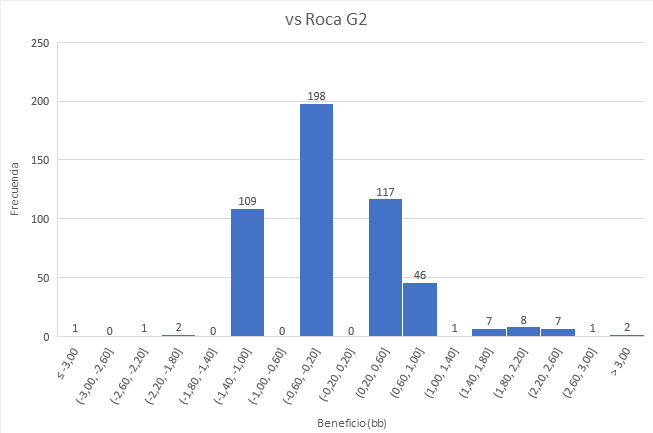
\includegraphics[width=1\textwidth]{figuras/AvRG2.png}   
\caption{Gráfica Algoritmo vs Roca (G2)}
\label{fig:AvRG2}
\end{figure}


\begin{figure}[h]
\centering
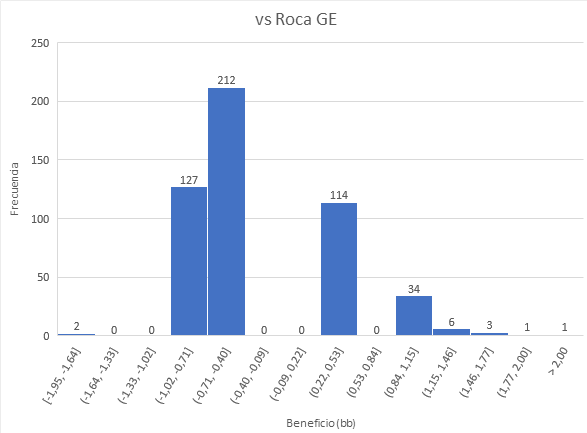
\includegraphics[width=1\textwidth]{figuras/AvRGE.png}   
\caption{Gráfica Algoritmo vs Roca (GE)}
\label{fig:AvRGE}
\end{figure}

\begin{figure}[h]
\centering
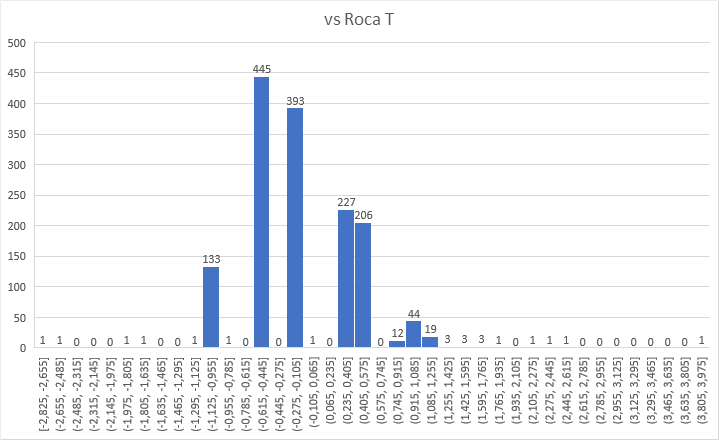
\includegraphics[width=1\textwidth]{figuras/AvRT.png}   
\caption{Gráfica Algoritmo vs Roca (T)}
\label{fig:AvRGT}
\end{figure}

Ahora se procede a estudiar el desarrollo de las partidas en cada uno de los conjuntos de los datos, estudiando primero el número de victorias generales, el número de partidas que han acabado en una determinada ronda (y el desglose de victorias/derrotas de esas partidas), así como calcular el porcentaje de victorias respecto a las rondas que acaban en esa ronda.


\begin{longtable}[c]{lrrrr}
\hline
Algoritmo vs Roca & G1 & G2 & GE & T \\ \hline
Nº Partidas & 500 & 500 & 500 & 1500 \\ 
Nº Victorias & 175 & 189 & 159 & 523 \\ 
Nº Derrotas & 325 & 311 & 341 & 977 \\ 
Partidas Fin Preflop & 378 & 389 & 400 & 1167 \\ 
Nº Victorias preflop & 79 & 99 & 86 & 264 \\ 
Nº Derrotas Preflop & 299 & 290 & 314 & 903 \\ 
Partidas Fin Flop & 115 & 104 & 94 & 313 \\ 
Nº Victorias Flop & 92 & 85 & 70 & 247 \\ 
Nº Derrotas Flop & 23 & 19 & 24 & 66 \\ 
Partidas Fin Turn & 5 & 6 & 5 & 16 \\ 
Nº Victorias Turn & 3 & 4 & 2 & 9 \\ 
Nº Derrotas Turn & 2 & 2 & 3 & 7 \\ 
Partidas Fin River & 1 & 1 & 0 & 2 \\ 
Nº VictoriasRiver & 1 & 1 & 0 & 2 \\ 
Nº Derrotas River & 0 & 0 & 0 & 0 \\ 
Partidas Fin Showdown & 1 & 0 & 1 & 2 \\ 
Nº Victorias Swodown & 0 & 0 & 1 & 1 \\ 
Nº Derrotas Showdown & 1 & 0 & 0 & 1 \\ \hline
\caption{Desglose de las partidas contra Roca}
\label{tab:PlaysR}
\end{longtable}

\begin{longtable}[c]{lrrrr}
\hline
\% Victoria vs Roca & G1 & G2 & GE & T \\ \hline
General & 35,000\% & 37,800\% & 31,800\% & 34,867\% \\ 
Preflop & 20,899\% & 25,450\% & 21,500\% & 22,622\% \\ 
Flop & 80,000\% & 81,731\% & 74,468\% & 78,914\% \\ 
Turn & 60,000\% & 66,667\% & 40,000\% & 56,250\% \\ 
River & 100,000\% & 100,000\% & - & 100,000\% \\ 
Showdown & 0,000\% & - & 100,000\% & 50,000\% \\  \hline
\caption{Porcentajes de victoria Algoritmo vs Roca (Desglose por rondas)}
\label{tab:winrateR}
\end{longtable}

El resultado final del enfrentamiento contra el patrón Roca es $-0.13481667\pm0.55795976$ $\frac{bb}{partida}$.

\vspace{5mm} %5mm vertical space

Cabe destacar que en la segunda toma de datos, no se llegó al Showdown en ninguna partida, mientras que en GE la única que se llegó a River, se continuó hasta el Showdown, por lo que ningua termino en River tampoco.

Si bien en el caso del Maniaco se encontraba con una reseñable mejora de GE con respecto de G1 y G2, no ocurre lo mismo en el caso contra Roca. En este caso se tiene, tanto una bajada de la media como de $Q_2$. Si bien es cierto estos datos por separado no tienen por qué ser un mal indicio, nos encontramos un descenso de la desviación (centralizando más los datos en torno a la media) y un descenso de las victorias de la ronda (al igual que no se encuentra ninguna mejoría de rondas que se llega hasta el Showdown). 


\clearpage


\subsubsection{Algoritmo vs Calling Station}

Se procede a desarrollar el resultado de las dos iteracciones contra Calling Station, empezando por los resultados de beneficio

\begin{longtable}[c]{lrrrr}
\hline
Algoritmo vs Calling Station & G1 & G2 & GE & T \\ \hline
$\bar{x}$ & -0,33416834 & -0,315 & -0,3085 & -0,21091667 \\ 
$\sigma$ & 1,12701073 & 1,07291426 & 0,84380255 & 0,67335509 \\ 
$\sigma^2$ & 1,2701532 & 1,151145 & 0,71200275 & 0,45340708 \\ 
C.V. & -3,37258385 & -3,406077 & -2,73517846 & -3,19251724 \\ 
Q1 & -1,08380282 & -0,87428571 & -0,9629932 & -0,57929293 \\ 
Q2 & -0,72918782 & -0,5308377 & -0,35323944 & -0,42164948 \\ 
Q3 & 0,13241758 & 0,29922222 & 0,25288889 & 0,19530387 \\ \hline
\caption{Tabla Algoritmo vs Calling Station}
\label{tab:AvC}
\end{longtable}


\begin{figure}[h]
\centering
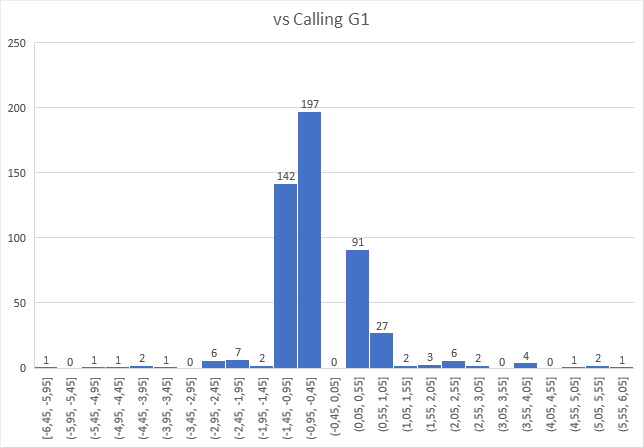
\includegraphics[width=1\textwidth]{figuras/AvCG1.png}   
\caption{Gráfica Algoritmo vs Calling Station (G1)}
\label{fig:AvRC1}
\end{figure}

\begin{figure}[h]
\centering
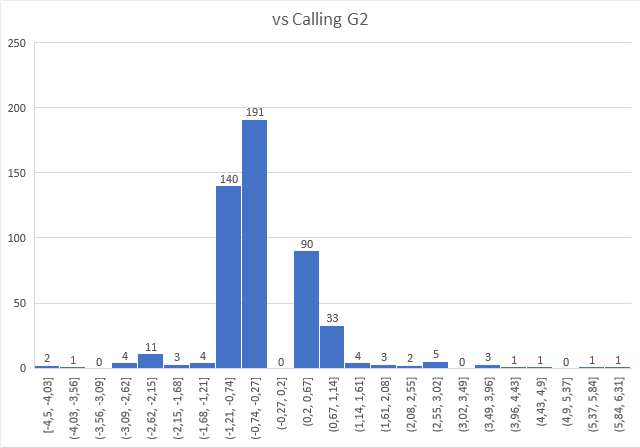
\includegraphics[width=1\textwidth]{figuras/AvCG2.png}   
\caption{Gráfica Algoritmo vs Calling Station (G2)}
\label{fig:AvRC2}
\end{figure}


\begin{figure}[h]
\centering
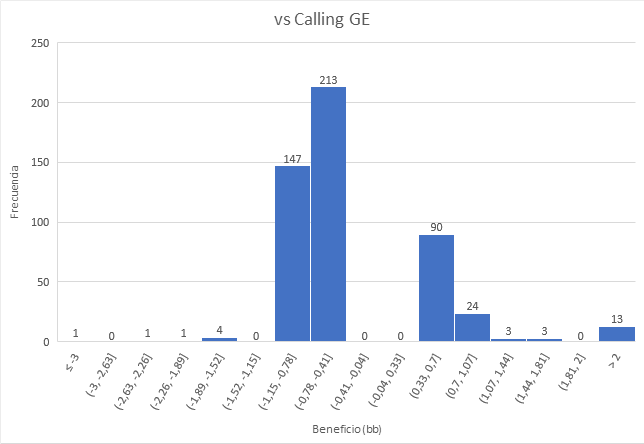
\includegraphics[width=1\textwidth]{figuras/AvCGE.png}   
\caption{Gráfica Algoritmo vs Calling Station (GE)}
\label{fig:AvRCE}
\end{figure}

\begin{figure}[h]
\centering
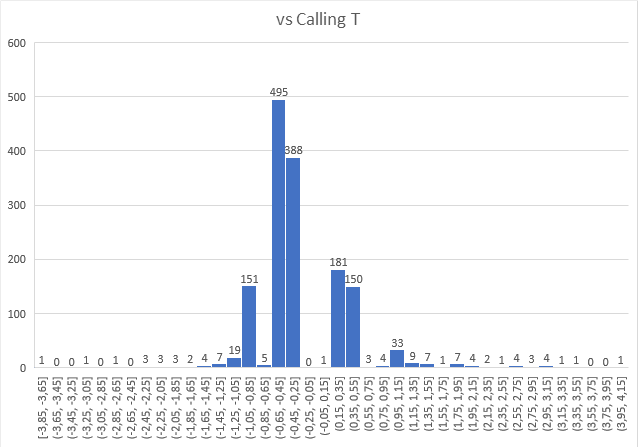
\includegraphics[width=1\textwidth]{figuras/AvCT.png}   
\caption{Gráfica Algoritmo vs Calling Station (T)}
\label{fig:AvRCT}
\end{figure}

Ahora se procede a estudiar el desarrollo de las partidas en cada uno de los conjuntos de los datos, estudiando primero el número de victorias generales, el número de partidas que han acabado en una determinada ronda (y el desglose de victorias/derrotas de esas partidas), así como calcular el porcentaje de victorias respecto a las rondas que acaban en esa ronda.


\begin{longtable}[c]{lrrrr}
\hline
Algoritmo vs Calling Station & G1 & G2 & GE & T \\ \hline
Nº Partidas & 500 & 500 & 500 & 1500 \\ 
Nº Victorias & 139 & 144 & 133 & 416 \\ 
Nº Derrotas & 360 & 356 & 367 & 1083 \\ 
Partidas Fin Preflop & 398 & 382 & 405 & 1185 \\ 
Nº Victorias preflop & 92 & 82 & 83 & 257 \\ 
Nº Derrotas Preflop & 306 & 300 & 322 & 928 \\ 
Partidas Fin Flop & 56 & 82 & 62 & 200 \\ 
Nº Victorias Flop & 26 & 45 & 30 & 101 \\ 
Nº Derrotas Flop & 30 & 37 & 32 & 99 \\ 
Partidas Fin Turn & 26 & 20 & 19 & 65 \\ 
Nº Victorias Turn & 12 & 10 & 8 & 30 \\ 
Nº Derrotas Turn & 14 & 10 & 11 & 35 \\ 
Partidas Fin River & 12 & 12 & 5 & 29 \\ 
Nº VictoriasRiver & 4 & 4 & 5 & 13 \\ 
Nº Derrotas River & 8 & 8 & 0 & 16 \\ 
Partidas Fin Showdown & 8 & 4 & 9 & 21 \\ 
Nº Victorias Swodown & 5 & 3 & 7 & 15 \\ 
Nº Derrotas Showdown & 2 & 1 & 2 & 5 \\ \hline
\caption{Desglose de las partidas contra Calling Station}
\label{tab:PlaysC}
\end{longtable}

\begin{longtable}[c]{lrrrr}
\hline
\% Victoria vs Calling Station & G1 & G2 & GE & Total \\ \hline
General & 27,800\% & 28,800\% & 26,600\% & 27,733\% \\ 
Preflop & 23,116\% & 21,466\% & 20,494\% & 21,688\% \\ 
Flop & 46,429\% & 54,878\% & 48,387\% & 50,500\% \\ 
Turn & 46,154\% & 50,000\% & 42,105\% & 46,154\% \\ 
River & 33,333\% & 33,333\% & 100,000\% & 44,828\% \\ 
Showdown & 62,500\% & 75,000\% & 77,778\% & 71,429\% \\ \hline
\caption{Porcentajes de victoria Algoritmo vs Calling Station (Desglose por rondas)}
\label{tab:winrateC}
\end{longtable}


El resultado final del enfrentamiento contra el patrón Calling Station es $-0.21091667\pm0.67335509$ $\frac{bb}{partida}$.

\vspace{5mm} %5mm vertical space

Aquí cabe destacar los valores de Showdown de G1, en el que hay 8 partidas que han llegado a Showdown, pero hay 5 victorias y 2 derrotas. Estos datos con correctos, pues la partida faltante resultó en empate, por lo que no hay ningún error en el procesado de datos.

Tras esta curiosidad sobre el empate, se procede a estudiar el conjunto de los datos de Calling Station. Siguiendo el hilo de resultados que se encontró en el apartado \ref{sec:pvp}, los resultados de los enfrentamientos con Calling Station son mixtos, aunque con tendencia positiva. Se aumenta ligeramente la media, se disminuye ligeramente la desviación y se puede apreciar una mejoría considerable de la mediana ($Q_2$), si bien los otros dos percentiles no se obtiene una mejora, pero tampoco se tiene un empeoramiento.
Por último, se observa que GE tiene un ligero menor número de victorias.

\clearpage

\subsection{Análisis del los datos por conjuntos}

En este apartado, se procede a estudiar los datos en conjunto, tomando como punto de estudio el origen de los datos. Es decir, se estudiarán los datos obtenidos del enfrentamiento contra los 3 algoritmos simultáneamente, tomando como un conjunto G1 y G2 ,como otro conjunto GE y por últimom T.

\subsubsection{Datos Previos a la modificación (G1 y G2)}

\begin{longtable}[c]{lr}
\hline
G1 y G2 & Valores \\ \hline
$\bar{x}$& -0,29861621 \\ 
$\sigma$ & 1,26776522 \\ 
$\sigma^2$& 1,60722864 \\ 
C.V.& -4,2454669 \\ 
$Q_1$ & -1,03119077 \\ 
$Q_2$ & -0,50274344 \\ 
$Q_3$ & 0,35380952 \\ \hline
\caption{Tabla Resultados comunes G1 y G2}
\label{tab:AGP}
\end{longtable}

\vspace{5mm} %5mm vertical space

El resultado final de los datos de G1 y G2 es $-0,29861621\pm1,26776522$ $\frac{bb}{partida}$.

\vspace{5mm} %5mm vertical space

\begin{figure}[h]
\centering
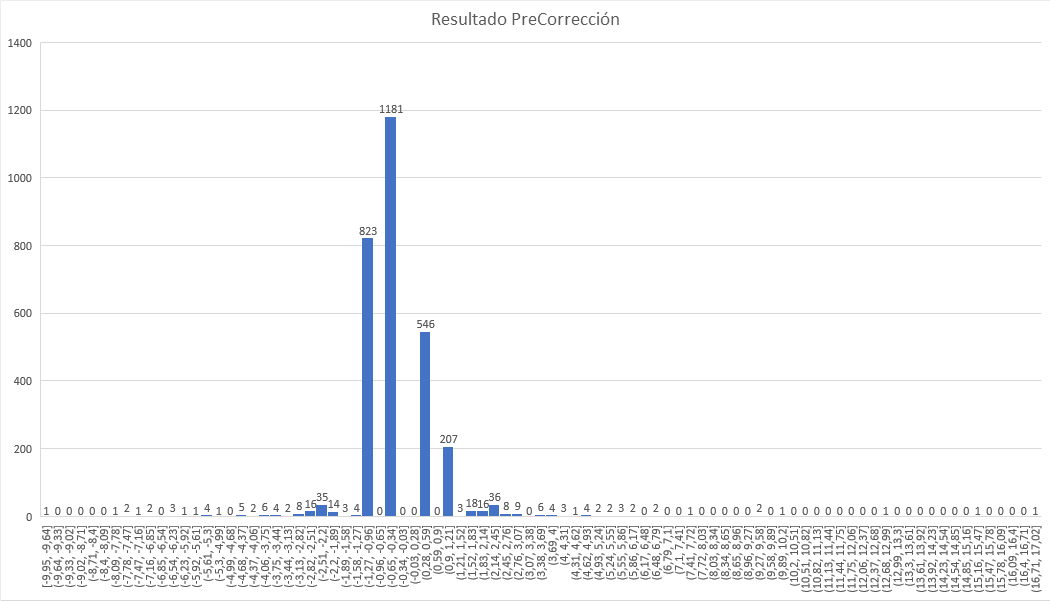
\includegraphics[width=1\textwidth]{figuras/AGP.png}   
\caption{Gráfica resultados Algoritmo G1 y G2}
\label{fig:AGP}
\end{figure}

\newpage

\subsubsection{Datos posteriores a la modificación (GE)}

\begin{longtable}[c]{lr}
\hline
GE & Valores \\ \hline
$\bar{x}$ & -0,28346667 \\ 
$\sigma$ & 1,57791845 \\ 
$\sigma^2$ & 2,48982665 \\ 
C.V. & -5,56650443 \\ 
$Q_1$ & -0,84511521 \\ 
$Q_2$ & -0,52945946 \\ 
$Q_3$ & 0,49235294 \\ \hline
\caption{Tabla Resultados GE}
\label{tab:AGC}
\end{longtable}

\vspace{5mm} %5mm vertical space

El resultado final de los datos de GE es $ -0,28346667\pm1,57791845$$\frac{bb}{partida}$.

\vspace{5mm} %5mm vertical space

\begin{figure}[h]
\centering
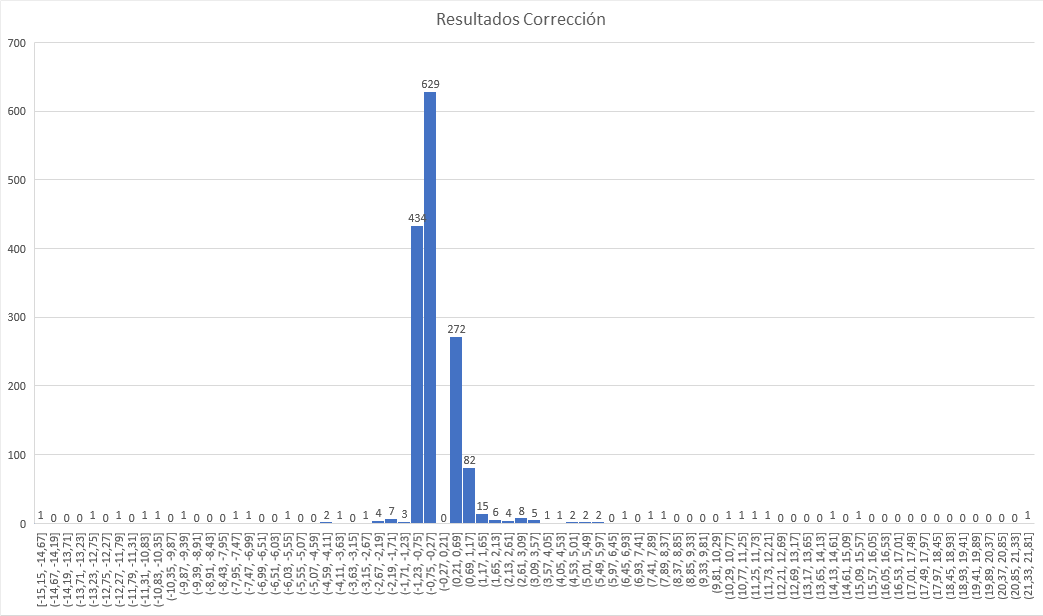
\includegraphics[width=1\textwidth]{figuras/AGC.png}   
\caption{Gráfica resultados Algoritmo GE}
\label{fig:AGC}
\end{figure}


\subsubsection{Datos totales (T)}

\begin{longtable}[c]{lr}
\hline
T & Valores \\ \hline
$\bar{x}$ & -0,19957213 \\ 
$\sigma$ & 1,06969216 \\ 
$\sigma^2$ & 1,14424131 \\ 
C.V. & -5,35992761 \\ 
$Q_1$ & -0,58161924 \\ 
$Q_2$ & -0,39856115 \\ 
$Q_3$ & 0,10397661 \\ \hline
\caption{Tabla Resultados T}
\label{tab:AGT}
\end{longtable}

El resultado final de los datos de T es  $-0,19957213\pm1,06969216$$\frac{bb}{partida}$.


\begin{figure}[h]
\centering
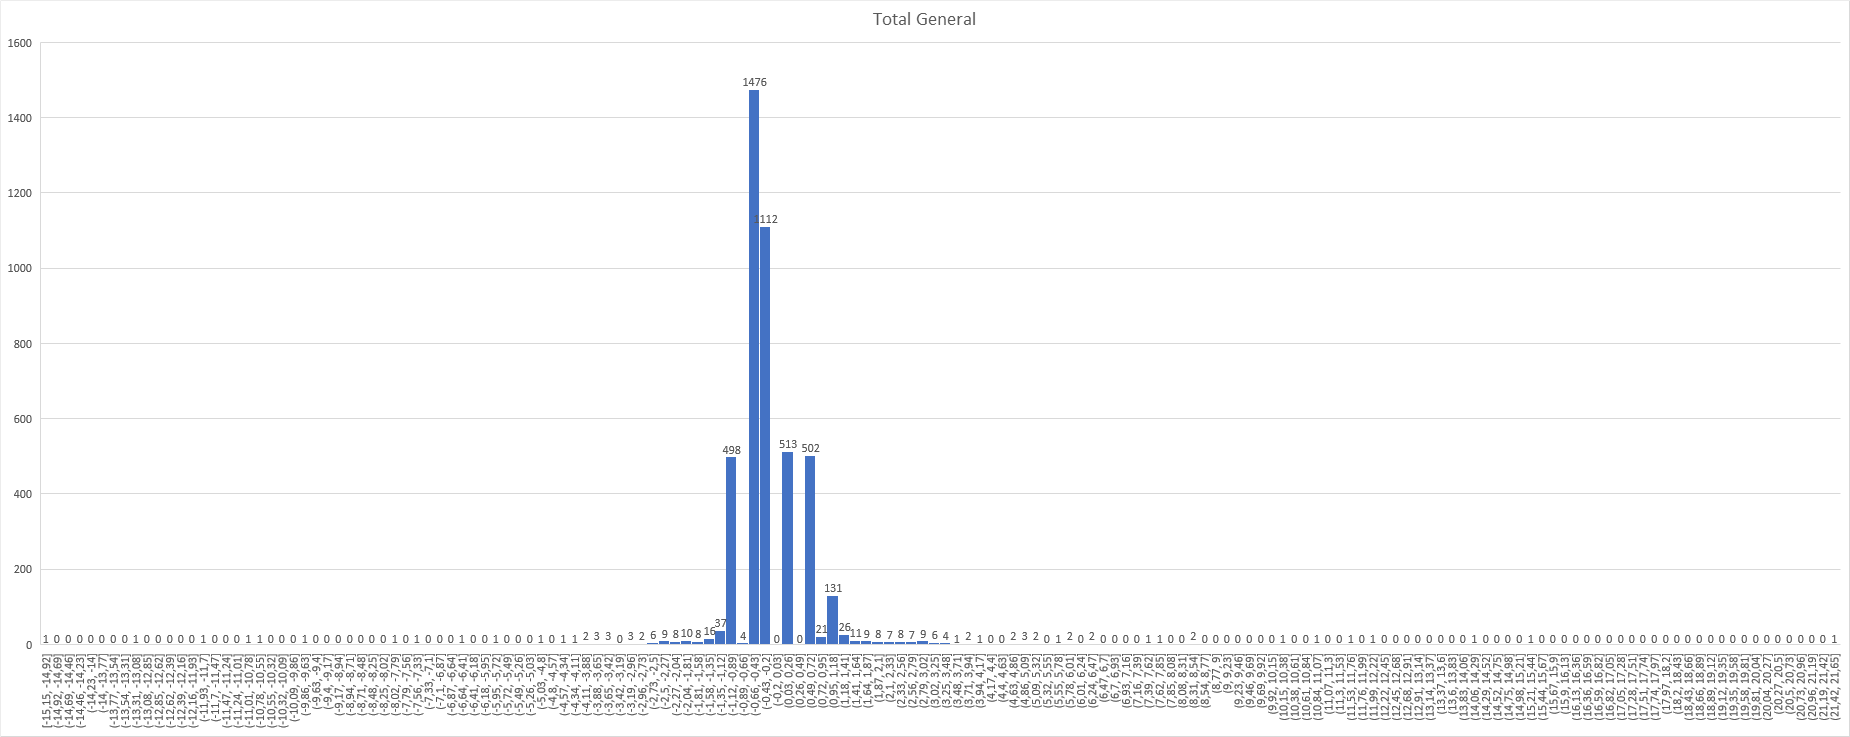
\includegraphics[width=1\textwidth]{figuras/AGT.png}   
\caption{Gráfica resultados Algoritmo T}
\label{fig:AGT}
\end{figure}

\newpage

\subsection{Tasa de victorias de los conjuntos}

\begin{longtable}[c]{lrrr}
\hline
Número de Partidas &  &  &  \\ \hline
Ronda & PreCorrección & Corrección & Total \\ \hline
Partida & 3000 & 1500 & 4500 \\ 
Preflop & 2363 & 1209 & 3572 \\ 
Flop & 474 & 212 & 686 \\ 
Turn & 103 & 44 & 147 \\ 
River & 38 & 8 & 46 \\ 
Showdown & 22 & 24 & 46 \\ \hline
\end{longtable}

\begin{longtable}[c]{lrrr}
\hline
Número de victorias totales &  &  &  \\ \hline
Ronda & PreCorrección & Correccoón & Total \\ \hline
Partida & 879 & 410 & 1289 \\ 
Preflop & 524 & 240 & 764 \\ 
Flop & 277 & 128 & 405 \\ 
Turn & 48 & 20 & 68 \\ 
River & 17 & 5 & 22 \\ 
Showdown & 13 & 17 & 30 \\ \hline
\end{longtable}

\begin{longtable}[c]{lrrr}
\hline
Tasa de Victorias &  &  &  \\ \hline
Ronda & PreCorrección & Correccoón & Total \\ \hline
Partida & 29,3000\% & 27,3333\% & 28,6444\% \\ 
Preflop & 22,1752\% & 19,8511\% & 21,3886\% \\ 
Flop & 58,4388\% & 60,3774\% & 59,0379\% \\ 
Turn & 46,6019\% & 45,4545\% & 46,2585\% \\ 
River & 44,7368\% & 62,5000\% & 47,8261\% \\ 
Showdown & 59,0909\% & 70,8333\% & 65,2174\% \\ \hline
\caption{Tasa de victorias por conjuntos}
\label{tab:winrateT}
\end{longtable}

\newpage

\section{Discusión preliminar de los datos}

En vista a estos resultados, salta a la vista que no se han obtenido los resultados esperados. Una cosa que estos resultados plantean sobre la mesa es que el diseño no funciona como se esperaba, por lo que es necesario analizar el diseño inicial y ver posibles causas del error.

Como se ha adelantado en el apartado \ref{sec:predisc}, tras hacer un rápido análisis a las dos primeras tandas de datos (G1 y G2) se detectó que había incoherencias entre las manos y algunas acciones que tomaba el algoritmo (sin considerar las que se pudieran considerar faroles), por lo que se decidió hacer una tercera medición eliminando esa aleatoriedad (dando lugar a GE). 

Una vez analizados los tres conjuntos de datos, la principal conclusión de los datos es que no hay una mejora significativa entre los datos previos a la corrección (G1 y G2)  y GE. Al tomar todos los datos en conjunto, el beneficio medio de GE es ligeramente mayor, con una desviación mayor también. Pero, en conjunto, esta mejor no es lo suficientemente significativa como para determinar que ese cambio haya mejorado el resultado del algoritmo.

A falta de más datos, no se puede afirmar que la causa de los malos resultados (o, al menos, la única causa) fuese la aleatoriedad de las tomas de decisiones del algoritmo. Por lo que es necesario replantearse cuál o cuáles pueden ser los otros elementos que pueden fallar.

Un factor que ha resultado llamativo ha sido la cantidad de manos que han acabado en la ronda del preflop, que ha sido tremendamente alta. Considerando que el 79,37\% de las manos han acabado en esta fase, es necesario considerar que el problema puede venir de esta fase. Este problema puede estar causado por algún error algorítmico a la hora de determinar las acciones durante el preflop.

 El problema no viene de que se hayan jugado solo el 20,62\% (pues, considerando los critrios de Sklansky-Malmuth y la fórmula de Chen, se estima que el número aproximado de manos que se pueden llegar a jugar son cerca del 24\%), sino que tan solo 8 de las 3572 rondas han tenido un beneficio absoluto mayor de 1. Es decir, que solo 8 de las 3572 manos que han acabado en interacción entre los jugadores. Lo que significa que de 4500 datos en los registros, el 79,2\% de esas manos tienen un beneficio de $\pm0.5$ o $\pm1$ $bb$.

Estos datos, por tanto, aparentan ser un indicio de que el origen de estos datos puede estar en el preflop. Por tanto, se procede al estudio de los datos de las partidas que no han acabado en el preflop, es decir, las partidas que han acabado en durante el postflop. 

\subsection{Análisis de los datos del postflop}

En esta sección se van a analizar el valor del beneficio de las partidas que no han acabado en el preflop. Lo primero que se ha hecho ha sido filtrar los datos que no han acabado en el preflop y, además, separar los que las partidas han sido de beneficio de $\pm1$ $bb$ (al no haber \textit{Antes}, la apuesta puede seguir hasta el Showdown con ambos jugadores siguiendo la apuesta sin variarla del valor de la ciega inicial) de las apuestas que han tenido un valor absoluto mayor.

De esta manera, se pueden recopilar los siguientes datos para cada conjunto de datos y para cada patrón:

\begin{itemize}
\item $N_{Total}$: Número total de rondas.
\item $N_{+1}$: Número de rondas con un beneficio de +1$bb$.
\item $N_{-1}$: Número de rondas con un beneficio de -1$bb$.
\item $N_{>1}$: Número de rondas con un beneficio mayor de +1$bb$.
\item $N_{<-1}$: Número de rondas con un beneficio menor de -1$bb$.
\item $N_{+}$: Número total de rondas con un beneficio positivo. En otras palabras,$N_{+}=N_{+1}+N_{>1}$.
\item $N_{-}$: Número total de rondas con un beneficio negativo. En otras palabras,$N_{-}=N_{-1}+N_{<-1}$.
\end{itemize}

Con estos datos, junto con el del valor de cada una de esas rondas, se proceden a calcular las diversas $\bar{x}$, $\sigma^2$ y $\sigma$, para cada uno de los conjuntos de datos y patrones, obteniendo las siguientes medidas:

\begin{itemize}
\item $\bar{x}_+$: Media de los valores positivos de un grupo de datos.
\item $\bar{x}_-$: Media de los valores negativos de un grupo de datos.
\item $\bar{x}_{+Total}$: Media de  los valores positivos de ese patrón.
\item $\bar{x}_{-Total}$: Media de los valores negativos  de ese patrón.
\item $\bar{x}_T$: Media de todos los valores de ese patrón.
\item $\sigma^2$ : Varianza de los valores del postflop de ese patrón.
\item $\sigma$ : Desviación tipica de los valores del postflop de ese patrón.
\end{itemize}


Estos son los resultados de este estudio.

\subsubsection{Algoritmo vs Maniaco}

\begin{longtable}[c]{lrrr}
\hline 
Algoritmo vs Maniaco & G1 & G2 & GE \\ \hline
$N_{Total}$ & 94 & 90 & 96 \\
$N_{+1}$& 13 & 7 & 21 \\
$N_{-1}$ & 33 & 30 & 31 \\
$N_{>1}$& 17 & 23 & 26 \\
$N_{<-1}$& 31 & 30 & 18 \\  
$N_{+}$ & 30 & 30 & 47 \\
$N_{-}$& 64 & 60 & 49 \\\hline
$\bar{x}_+$ & 2,77 & 4,10333333 & 4,20744681 \\
$\bar{x}_-$& -2,27421875 & -2,315 & -3,05714286 \\ \hline
\caption{Datos Postflop Algoritmo vs Maniaco}
\label{tab:DPFAvM}
\end{longtable}

Siendo estos los cálculos totales:

\vspace{5mm} %5mm vertical space

\begin{longtable}[c]{lr}
\hline 
Medida & Valor \\ \hline 
$\bar{x}_{+Total}$ & 3,77523364 \\
$\bar{x}_{-Total}$ & -2,51011561 \\
$\bar{x}_T$ & -0,10821429 \\
$\sigma^2$ & 19,1653962 \\
$\sigma$ & 4,37783008 \\  \hline
\caption{Medidas Postflop Algoritmo vs Maniaco}
\label{tab:MPFAvM}
\end{longtable}

El resultado final de los datos de Algoritmo vs Maniaco en el postflop es  $-0,10821429\pm4,37783008 $$\frac{bb}{partida}$.

\vspace{5mm} %5mm vertical space

\subsubsection{Algoritmo vs Roca}

\begin{longtable}[c]{lrrr}
\hline 
Algoritmo vs Roca & G1 & G2 & GE \\ \hline
$N_{Total}$& 122 & 111 & 100 \\
$N_{+1}$& 75 & 65 & 59 \\
$N_{-1}$ & 20 & 18 & 25 \\
$N_{>1}$& 21 & 25 & 14 \\
$N_{<-1}$& 6 & 3 & 2 \\
$N_{+}$& 96 & 90 & 73 \\
$N_{-}$& 26 & 21 & 27 \\ \hline
$\bar{x}_+$ & 1,25416667 & 1,32277778 & 1,10547945 \\
$\bar{x}_-$& -1,4 & -1,31666667 & -1,05925926 \\ \hline
\caption{Datos Postflop Algoritmo vs Roca}
\label{tab:DPFAvR}
\end{longtable}

Siendo estos los cálculos totales

\begin{longtable}[c]{lr}
\hline 
Medida & Valor \\ \hline 
$\bar{x}_{+Total}$ & 1,23610039 \\
$\bar{x}_{-Total}$ & -1,25202703 \\
$\bar{x}_T$ & 0,68318318 \\
$\sigma^2$ & 0,85923713 \\
$\sigma$ & 0,92695045 \\  \hline
\caption{Medidas Postflop Algoritmo vs Roca}
\label{tab:MPFAvR}
\end{longtable}


El resultado final de los datos de Algoritmo vs Roca en el postflop es  $ 0,68318318\pm 0,92695045 $$\frac{bb}{partida}$.

%\vspace{10mm} %5mm vertical space
\newpage

\subsubsection{Algoritmo vs Calling Station}

\begin{longtable}[c]{lrrr}
\hline 
Algoritmo vs Caling Station & G1 & G2 & GE \\ \hline
$N_{Total}$& 102 & 118 & 95 \\
$N_{+1}$& 26 & 42 & 31 \\
$N_{-1}$ & 33 & 34 & 38 \\
$N_{>1}$& 21 & 20 & 19 \\
$N_{<-1}$& 21 & 22 & 7 \\
$N_{+}$& 47 & 62 & 50 \\
$N_{-}$& 54 & 56 & 45 \\ \hline
$\bar{x}_+$ & 1,91808511 & 1,62822581 & 1,525 \\
$\bar{x}_-$& -1,7212963 & -1,58125 & -1,17777778 \\ \hline
\caption{Datos Postflop Algoritmo vs Calling Station}
\label{tab:DPFAvC}
\end{longtable}

Siendo estos los cálculos totales

\begin{longtable}[c]{lr}
\hline 
Medida & Valor \\ \hline 
$\bar{x}_{+Total}$ & 1,68144654 \\
$\bar{x}_{-Total}$ & -1,51290323 \\
$\bar{x}_T$ & 0,10428571 \\
$\sigma^2$ & 2,98798947 \\
$\sigma$ &1,72858019 \\  \hline
\caption{Medidas Postflop Algoritmo vs Calling Station}
\label{tab:MPFAvC}
\end{longtable}


El resultado final de los datos de Algoritmo vs Calling Station en el postflop es  $0,10428571\pm 1,72858019 $$\frac{bb}{partida}$.

\vspace{5mm} %5mm vertical space


\subsubsection{Total de los patrones}

Teniendo en cuenta que los valores $N_i$ correspondientes a esta tabla son la suma de esos valores en cada una de las tablas de los tres patrones, solo se van a incluir en esta los valores calculados.

\begin{longtable}[c]{lrrr}
\hline 
Total & G1 & G2 & GE \\ \hline
$\bar{x}_+$ & 1,24756944 & 1,71021898 & 2,01404959 \\
$\bar{x}_-$& -1,32569444 & -1,26350365 & -1,11900826 \\ \hline
\caption{Datos Postflop Totales}
\label{tab:DPFT}
\end{longtable}

\vspace{5mm} %5mm vertical space

\begin{longtable}[c]{lr}
\hline 
Medida & Valor \\ \hline 
$\bar{x}_{+Total}$ & 1,2427619 \\
$\bar{x}_{-Total}$ & -1,24228856 \\
$\bar{x}_T$ &0,16610991 \\
$\sigma^2$ & 7,15948169 \\
$\sigma$ &2,67572078 \\  \hline
\caption{Medidas Postflop Totales}
\label{tab:MPFT}
\end{longtable}

El resultado final del total de los datos en el postflop es  $0,16610991\pm 2,67572078 $$\frac{bb}{partida}$.

\subsubsection{Análisis de los resultados}

Se va a elaborar una pequeña tabla con todos estos valores, así como los valores obtenidos en el apartado \ref{sec:AvP}, para un estudio mucho más cómodo, permitiendo una mejor comparación entre los distintos valores.

\begin{longtable}[c]{lrr}
\hline 
 & Resultado Postflop & Resultado General \\ \hline
Algoritmo vs Maniaco & $-0,10821429\pm4,37783008 $ &  $-0.3764667\pm1.982518$ \\
Algoritmo vs Roca & $ 0,68318318\pm 0,92695045 $  &  $-0.13481667\pm0.55795976$  \\
Algoritmo vs Calling Station &$0,10428571\pm 1,72858019 $  & $-0.21091667\pm0.67335509$ \\
Total & $0,16610991\pm 2,67572078$ & $-0,19957213\pm1,06969216$\\ \hline
\caption{Datos Postflop Totales}
\label{tab:DPFT}
\end{longtable}

De esta comparación, se puede observar una mejoría de tanto la $\bar{x}$ en todos los casos, siendo especialmente significativo el caso del enfrentamiento de Algoritmo vs roca, donde es el que más incremento se obtiene (siendo este incremento+0.817999985 $\frac{bb}{partida}$). Por otro lado, el valor de $\sigma$ también se incrementa para todos los casos.

Por otro lado, se puede hacer una comparación también de partidas ganadas. De las tablas, se puede obtener que en el postflop se da un incremento notable del ratio de victorias del algoritmo frente a la partida total (56,57\% en el postflop frente al 28,64\% del total de las partidas). 

Si bien este dato aparenta ser significativamente mejor, al comparar el incremento del ratio de victorias con el incremento de la $\bar{x}$ obtenida en el total de los datos, se puede observar que el aumento de la $\bar{x}$ no se incrementa tanto como lo hace el ratio de victorias. Este dato es curioso, puesto que si se toma solamente el ratio de victorias como indicador, en esta situación estaríamos ante un crecimiento de casi el doble del ratio de victorias, pero eso no se traslada a los beneficios, pues es un dato bastante menor (se produce un incremento del 120\% de la media frente al incremento del 197\% del ratio de victorias). 

Esto tiene una interpretación clara: los resultados, una vez se alcanza el flop, tienden a ser mejores, pero también más variables, permitiendo tanto ganar más dinero como perder más dinero. También aumenta el número de victorias, pero no aumenta tanto el beneficio obtenido. 
 En otras palabras, los datos arrojan que, cuanto mayor sea la duración de una partida (en lo que se refiere a rondas de apuestas), el algoritmo gana más partidas, pero no gana tanto dinero como pudiera parecer.


\section{Discusión final de los datos}
\label{sec:discusion}

Con el estudio hecho en el apartado anterior, se ha detectado que un punto de inflexión: hay un gran salto de la eficacia del algoritmo del preflop a las rondas posteriores (Flop, Turn y River), llegando a obtener una ganancia media de $0,16610991\pm 2,67572078 $$\frac{bb}{partida}$. 
Pero, considerando que la ganancia media del algoritmo en una partida en general es de $-0,19957213\pm1,06969216$$\frac{bb}{partida}$, se puede deducir que el rendimiento no es el esperado ni el adecuado. Si bien estos datos pueden deberse a mero azar, se puede asumir también que el planteamiento inicial no era del todo adecuado.

Después del análisis de los datos (tanto a nivel general como a nivel del postflop), se pueden delimitar los focos de los fallos de diseño que causan que, a nivel general, el rendimiento no sea el esperado:

\begin{itemize}
\item \textbf{El número de manos jugadas en el preflop es demasiado bajo:} Esta afirmación tiene tanto un punto que la rechaza como un punto que la respalda. Si bien es cierto que, de acuerdo con los criterios de Sklansky-Malmuth \cite{sklansky} como en la fórmula de Chen \cite{krieger}, el número de manos jugadas debe estar en el margen del 17-26\% aproximadamente , estando en un 20,64\% es un dato que aún puede mejorar. Además, si se consideran los grupos 7 y 8 del criterio de Sklansky-Malmuth, este porcentaje podría incrementarse hasta un 42\% de las manos jugadas.
\item \textbf{El beneficio obtenido en el postflop no es lo suficientemente alto como para compensar las apuestas perdidas en el preflop:} Este razonamiento viene de que, a pesar de ganar más partidas, el beneficio por partida que se alcanza el Flop no se incrementa tanto como para conseguir que la $\bar{x}$ general mejore de manera significativa. Esto se traduciría como la fórmula de cálculo de acción después del preflop no tiene el rendimiento esperado.
\end{itemize}

El razonamiento lógico a pensar es que ambos focos tengan algo que ver con este rendimiento. Por lo cual, los puntos donde es adecuado el diseño y el planteamiento del algoritmo, se encontrará en, al menos, uno de esos focos, dado que ambos factores afectan al beneficio medio por partida.
Con los datos que se tiene actualmente, no se pueden aislar con más precisión qué factor o factores del planteamiento y/o del diseño del algoritmo provocan estos resultados.

 Para llegar a corregir este diseño, sería necesario tomar una mayor cantidad de datos, hacer pruebas cambiando las condiciones y las especificaciones, así como ir variando los distintos valores (como las fórmulas de los cambios de acción o el modelado de los patrones) para intentar detectar el origen u orígenes de este fallo de diseño y, posteriormente, corregirlo en pos de obtener un algoritmo óptimo.